\section{The algebraic Tate diagonal}

Let $p$ be a prime and $\cyc_p$ be the cyclic group of order $p$. 

\begin{definition} We denote by $T_p$ the functor
\[
T_p\coloneqq (-\otimes \overset{p}{\cdots}\otimes -)^{t\cyc_p} \colon \mathcal D(\Fp)\to \mathcal D(\Fp).
\]
Explicitly, given $V$ in $\mathcal D(\Fp)$, $T_pV$ is the $\cyc_p$-Tate construction of the chain complex of $\Fp[\cyc_p]$-modules $V^{\otimes p}$, with $\cyc_p$-action given by permuting the factors.
\end{definition}

\begin{example}
Taking $M=\k$, with the trivial G action...
\end{example}

Let $C$ be a chain complex and set $M = C^{\otimes p}$. A model for its Tate construction is given by
\[
(C^{\otimes p})^{t\cyc_p} \cong \widehat W(p)\otimes_{\cyc_p} C^{\otimes p}.
\]

A result of Nikolaus and Scholze~\cite{??} shows that in $\sD(\Z)$ there is no natural chain map
\[
C \longrightarrow (C^{\otimes p})^{t\cyc_p}
\]
inducing a nontrivial map on homology.

Nevertheless, one can define the map
\[
\Delta^t(p)\colon H_*(C)\longrightarrow H_*\big((C^{\otimes p})^{t\cyc_p}\big)
= H_*\big(\widehat W(p)\otimes_{\cyc_p} C^{\otimes p}\big)
\]
by sending a class $[x]$ in degree $n$ to
\[
[x] \longmapsto [\,e_{(1-p)n}\otimes_{\cyc_p} (x\otimes \overset{_{(p)}}{\cdots} \otimes x)\,].
\]
We refer to $\Delta^t(p)$ as the \defn{algebraic Tate diagonal}.

\begin{lemma}
The algebraic Tate diagonal is $\bF_p$-linear.
\end{lemma}
\begin{proof}
First we check scalar multiplicativity, let $a\in\bF_p$ and $[x]\in H_n(C)$.
\[
\Delta^t(p)(a[x])=[e_{(1-p)n}\ot_{\cyc_p}(ax)^{\ot p}]=a^p[e_{(1-p)n}\ot_{\cyc_p}x^{\ot p}]=a\Delta^t(p)([x]),
\]
where the last equality holds in $\bF_p$ due to Fermat's little theorem.

Now, for aditivity, let $[x]$ and $[y]\in H_n(C)$. We have
\[
\Delta^t(p)([x]+[y])=[e_{(1-p)n}\ot_{\cyc_p}(x+y)^{\ot p}].
\]
The term $(x+y)^{\ot p}$ is a sum of $2^p$ terms, corresponding to the set of all possible words of length $p$ using the leters $x$ and $y$. The cyclic group acts on this set by permutation, and there are two types of orbits: those consisting of a single element and those with $p$ elements. There are two orbits with a single element, corresponding to $x^{\otimes p}$ and $y^{\otimes p}$ respectively. Let ${\bf w}_1,\dots, {\bf w}_{(2^{p}-2)/p}$ be representatives of the remaining orbits. Thus, we can write
\[
[e_{(1-p)n}\ot_{\cyc_p}(x+y)^{\ot p}]=[e_{(1-p)n}\ot_{\cyc_p}x^{\ot p}]+[e_{(1-p)n}\ot_{\cyc_p}y^{\ot p}]+\sum_{i=1}^{(2^{p}-2)/p}[e_{(1-p)n}\ot_{\cyc_p}N{\bf w}_i],
\]
but 
\[
e_{(1-p)n}\ot_{\cyc_p}N{\bf w}_i=Ne_{(1-p)n}\ot_{\cyc_p}{\bf w}_i=de_{(1-p)n+1}\ot_{\cyc_p}{\bf w}_i=d(e_{(1-p)n+1}\ot_{\cyc_p}{\bf w}_i),
\]
where the second equality holds because $(1-p)n+1$ is an odd number for $p$ prime (and $de_j=Ne_{j-1}$ for any $j$ if $p=2$), and the last equality holds since $x$ and $y$ are cycles. This means that the term $\sum_{i=1}^{(2^{p}-2)/p}[e_{(1-p)n}\ot_{\cyc_p}N{\bf w}_i]$ vanishes, and so
\[
\Delta^t(p)([x]+[y])=\Delta^t(p)([x])+ \Delta^t(p)([y]).\qedhere
\]
\end{proof}

\subsection{Monoidality}

Let $H \colon \sD(\Fp)\to \text{GrVect}_\Fp$ denote the homology functor. It is a lax monoidal functor: for chain complexes $C$ and $D$, the Künneth map defines a morphism
\[
\kappa \colon H(C)\otimes H(D)\longrightarrow H(C\otimes D),
\]
which is natural in $C$ and $D$.

Let $H^t(p)$ denote the composite
\[
\sD(\Fp) \xra{(-)^{\otimes p}} \sD(R) \xra{(-)^{t\cyc_p}} \sD(\Fp) \xra{H} \text{GrVect}_\Fp.
\]
This is again a lax monoidal functor. Indeed, there is a natural morphism
\[
\mu\circ \kappa\colon H\big(\widehat W\otimes_{\cyc_p} C^{\otimes p}\big)\otimes H\big(\widehat W\otimes_{\cyc_p} D^{\otimes p}\big)
\longrightarrow H\big(\widehat W\otimes_{\cyc_p} (C\otimes D)^{\otimes p}\big),
\]
where
\[
\mu\colon H\big((\widehat W\otimes_{\cyc_p} C^{\otimes p})\otimes (\widehat W\otimes_{\cyc_p} D^{\otimes p})\big)
\longrightarrow H\big(\widehat W\otimes_{\cyc_p} (C\otimes D)^{\otimes p}\big)
\]
is induced by the assignment
\[
[(\rho^a e_i\otimes_{\cyc_p} \mathbf{c})\otimes (\rho^b e_j\otimes_{\cyc_p} \mathbf{d})]
\longmapsto
[\,e_{i+j}\otimes_{\cyc_p} \mathrm{Sh}(\rho^{-a}\mathbf{c}, \rho^{-b}\mathbf{d})\,],
\]
for $\mathbf{c}=c_1\otimes\cdots\otimes c_p \in C^{\otimes p}$ and $\mathbf{d}=d_1\otimes\cdots\otimes d_p \in D^{\otimes p}$. Here $\mathrm{Sh}$ denotes the shuffle map $C^{\otimes p}\times D^{\otimes p}\to(C\otimes D)^{\otimes p}$ given by
\[
((c_1\otimes\cdots\otimes c_p), (d_1\otimes\cdots\otimes d_p))
\longmapsto
(c_1\otimes d_1)\otimes\cdots\otimes (c_p\otimes d_p).
\]

The following diagram commutes for all chain complexes $C$ and $D$:
\begin{center}
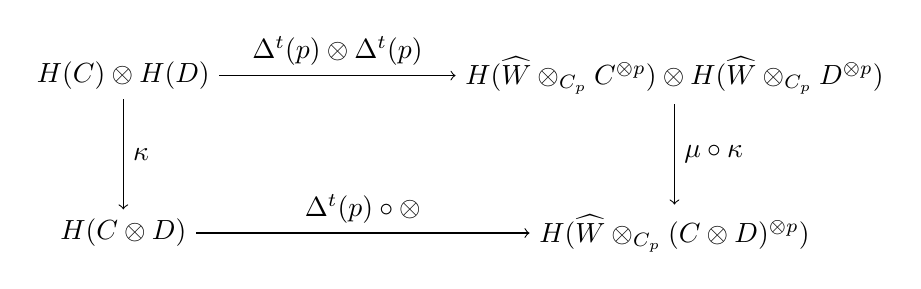
\begin{tikzpicture}
\node (a) at (-3,2){$H(C)\otimes H(D)$};
\node (b) at (4,2){$H(\widehat W\otimes_{C_p} C^{\otimes p})\otimes H(\widehat W\otimes_{C_p} D^{\otimes p})$};
\node (c) at (-3,0){$H(C\otimes D)$};
\node (d) at (4,0){$H(\widehat W\otimes_{C_p} (C\otimes D)^{\otimes p})$};
%
\draw[->](a) -- node[above]{$\Delta^t(p)\otimes \Delta^t(p)$}(b);
\draw[->](a)--node[right]{$\kappa$}(c);
\draw[->](b)--node[right]{$\mu\circ\kappa$}(d);
\draw[->](c)--node[above]{$\Delta^t(p)\circ \otimes$}(d);

\end{tikzpicture}
\end{center}


\begin{lemma}
The algebraic Tate diagonal defines a monoidal natural transformation
\[
\Delta^t(p)\colon H \longrightarrow H^t(p).
\]
\end{lemma}
